The goal of this laboratory activity was to implement a simple algorithm for line following using our TurtleBot. The robot was equipped with a line sensor array, which allowed it to detect the presence of a line on the ground.
The line sensor array consisted of multiple infrared sensors that could detect the contrast between the line and the background surface. In our case the sensor was placed on the front side of the rover. 
The robot was programmed to follow the line by adjusting its speed and direction based on the sensor readings. 
In particular we implemented two algorithms: 
\begin{itemize}
    \item A simple initial algorithm that used the sensor readings to determine whether the robot was on the line, off to the left, or off to the right. Based on this information, the robot adjusted its speed and direction to stay on the line.
    \item A more advanced algorithm, i.e. the yaw controller, which used the sensor readings to calculate the error in the robot's position relative to the line. The robot then adjusted its speed and direction based on this error, allowing it to follow the line more accurately.
\end{itemize}

\subsection{Theoretical background}
In this section we will describe the model of the robot used in this laboratory activity. In particular, we will focus on the line sensor array and on the kinematic model of the robot.

\subsubsection{Line sensor array}
Our line sensor array consisted of the Pololu QTR reflectance sensors, whose modo operandis is described in Section~\ref{sec:line_sensor}. 
We remind that the microcontroller can read from the reflectance sensor by interfacing with a port expander, which is connected to the sensors via an I2C bus connection.
An important parameter of the sensor line is the pitch, which is the distance between two adjacent sensors. The list below summarizes the main parameters of the sensor array used in this laboratory activity:
\begin{table}[H]
    \centering
    \begin{tabular}{cc}
        \toprule
        \textbf{Parameter} & \textbf{Value} \\
        \midrule
        Sensor output & digital \\
        Number of sensors ($N$) & 8 \\
        Pitch ($P$) & 8 mm or 0.008 m \\
        \bottomrule
    \end{tabular}
    \caption{}
\end{table}

Furthermore, we worked under the following assumptions:
\begin{itemize}
    \item The line is wide enough to activate at least two sensors at a time;
    \item There is always at least one sensor that is not active;
    \item A line is detected if one or more adjacent sensors are activate.
\end{itemize}

For our goal, it was important to define the line tracking error $e_{SL}$, which is the distance between the center of the robot and the center of the line, i.e.
\begin{equation}
    f(x) = \left\{
    \begin{array}{ll}
        e_{SL} = 0 & \text{when the line is at the center} \\
        e_{SL} > 0 & \text{when the line is on the left side of the sensor} \\
        e_{SL} < 0 & \text{when the line is on the right side of the sensor}
    \end{array}
    \right.
\end{equation}
We define the sequence of active sensors as:
\begin{equation}
    b_n = 
    \begin{cases}
        1 & \text{if sensor $n$ is active} \\
        0 & \text{if sensor $n$ is not active}
    \end{cases}
\end{equation}
and the distance between the sensor at position $n$ and the center of the sensor array as:
\begin{equation}
    \label{eq:lambda_n}
    \lambda_n = \left( \frac{N-1}{2} - n \right) \, P, \quad n = 0, \ldots, N-1
\end{equation}
The line tracking error can then be computed as the weighted average of the distances of the activate sensors from the center of the sensor array, i.e.:
\begin{equation}
    \label{eq:e_sl}
    e_{SL} = \frac{\sum_{n=0}^{N-1} b_n \lambda_n}{\sum_{n=0}^{N-1} b_n} 
\end{equation}

\begin{figure} [H]
    \centering
    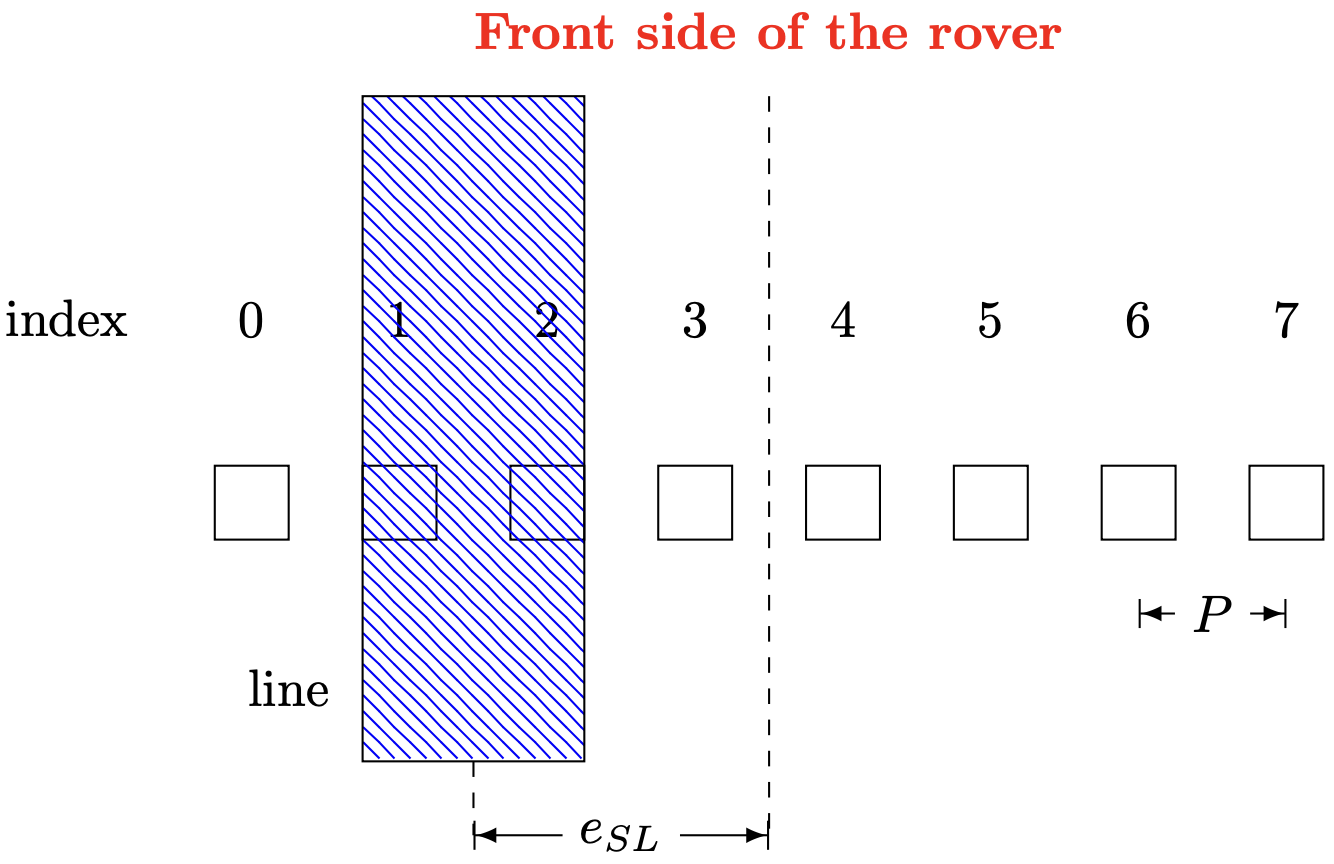
\includegraphics[width=0.7\textwidth]{lab4/figures/e_sl.png}
    \caption{Line tracking error}
    \label{fig:line_tracking_error}
\end{figure}

\subsubsection{Kinematic model}
In Figure~\ref{fig:kinematic_model} is shown the kinematic model of the robot used in this laboratory activity, whose mechanical parameters are reported in Table~\ref{tab: mech_param}.
\begin{table}[H]
    \centering
    \begin{tabular}{cc}
        \toprule
        \textbf{Parameter}  & \textbf{Value} \\
        \midrule
        Wheel distance ($D$) & 0.165 m \\
        Distance between the sensor and the vehicle's centre ($H$) & 0.085 m \\
        Wheel radius ($r$) & 0.034 m \\
        \bottomrule 
    \end{tabular}
    \caption{}
    \label{tab: mech_param}
\end{table}
The robot has two wheels that can be controlled independently, and in the following we assume a pure roll condition, i.e. the wheels do not slip on the ground.
The relations that connect the linear velocity of the wheels $V_l$ and $V_r$ with the angular velocities of the left and right wheels $\omega_l$ and $\omega_r$ are:
\begin{equation}
    V_r = r \cdot \omega_r, \quad V_l = r \cdot \omega_l
\end{equation}
where $r$ is the radius of the wheels.
The rotation of the robot is around the Instantaneous Center of Rotation (ICR), which is the point where the robot is not moving. The ICR is located at a distance $R$ from the center of the robot.
While, the distance between the two wheels is denoted as $D$. It holds that:
\begin{equation}
    V_r = \omega(R+D/2), \quad V_l = \omega(R-D/2)
\end{equation}
and by subtracking these two equations we obtain:
\begin{equation}
    \omega = \frac{V_r - V_l}{D}
\end{equation}

The angle $\psi$ between the global frame and the robot's frame is equal to the angle between the x-axis and the line connecting the ICR to the center of the robot, i.e. $\omega$.
Therefore, the yaw rate of the robot is equal to $\omega$, i.e.:
\begin{equation}
    \dot{\psi} = \frac{V_r - V_l}{D}
\end{equation}
Then, the linear velocity of the robot can be computed as the average of the linear velocities of the two wheels, i.e.:
\begin{equation}
    V = \frac{V_r + V_l}{2}
\end{equation}
And, finally, we derive the formulas which take into account both the longitudinal speed of the wheels and the yaw rate:
\begin{equation}
\begin{cases}
    V_r = V + \dot{\psi} \frac{D}{2} \\
    V_l = V - \dot{\psi} \frac{D}{2}
\end{cases}
\end{equation}
from which it immediately follows
\begin{equation}
\begin{cases}
    \label{eq:omega}
    \omega_r = \frac{V + \dot{\psi} \frac{D}{2}}{r} \\
    \omega_l = \frac{V - \dot{\psi} \frac{D}{2}}{r}
\end{cases}
\end{equation}
\begin{figure} [H]
    \centering
    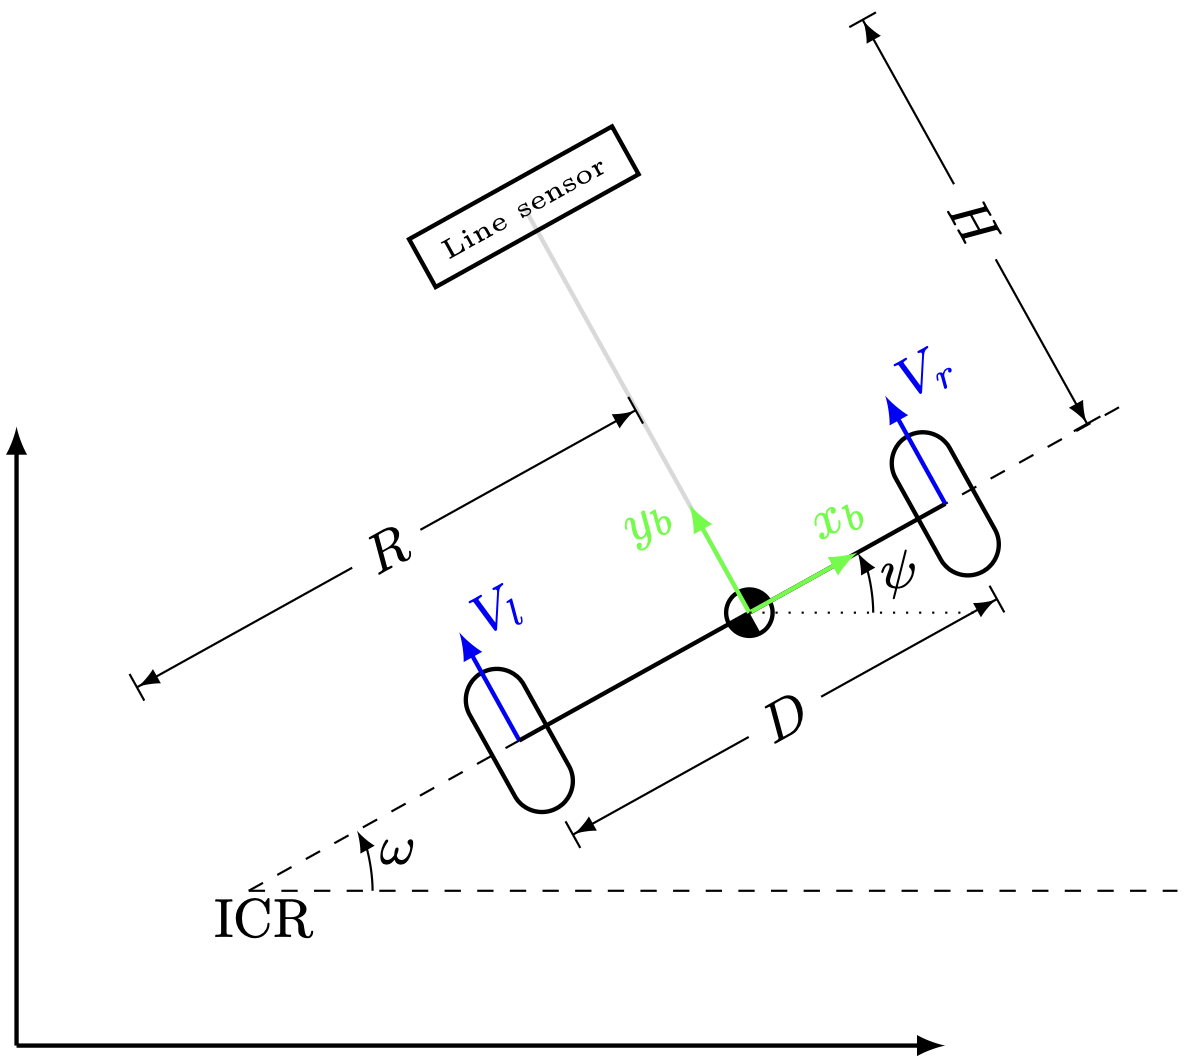
\includegraphics[width=0.6\textwidth]{lab4/figures/kinematic_model.png}
    \caption{Kinematic model}
    \label{fig:kinematic_model}
\end{figure}

\subsubsection{Yaw error}
At this point, we need to define the yaw error, which is the difference between the desired yaw angle ($\psi_{ref}$) and the actual yaw angle ($\psi$) of the robot. The yaw error can be expressed as:
\begin{equation}
    \psi_{err} = \psi_{ref} - \psi
\end{equation}

The relationship between the yaw error and the line tracking error can be expressed as follows:
\begin{equation}
    \label{eq:psi_err}
    \psi_{err} = \arctan\left(\frac{e_{SL}}{H}\right) \approx \frac{e_{SL}}{H}
\end{equation}
Where the last equation exploits the small angle approximation, which is valid for small values of $e_{SL}$.

\subsection{System configuration}
This section describes the hardware components, architecture, and configuration of the mobile robot system used for yaw control and line following.

The hardware components are the same described in Section~\ref{sec:system_configuration}.

The control structure of the system, used for the implementation of the yaw controller, is divided into two layers:
\begin{itemize}
    \item Low-level layer: responsible for maintaining the desired velocities of the left and right wheels using PI controllers.
    \item High-level layer: computes the yaw error from the sensor data and applies a proportional correction to the wheel speed reference, effectively steering the robot back onto the path.
\end{itemize} 

When the robot deviates from the center of the line, the yaw error increases. 
The proportional yaw controller reacts by adjusting the difference between the left and right wheel speeds, thereby rotating the robot toward the line. 
This hierarchical control scheme ensures smooth and responsive tracking of the line.

For the design of the yaw controller, we considered as input the yaw error ($\psi_{err}$) and the output was the control signal for the robot's wheels, i.e. the yaw rate ($\dot{\psi}$), as shown in Figure~\ref{fig:yaw_controller}.
\begin{figure}[H]
    \centering
    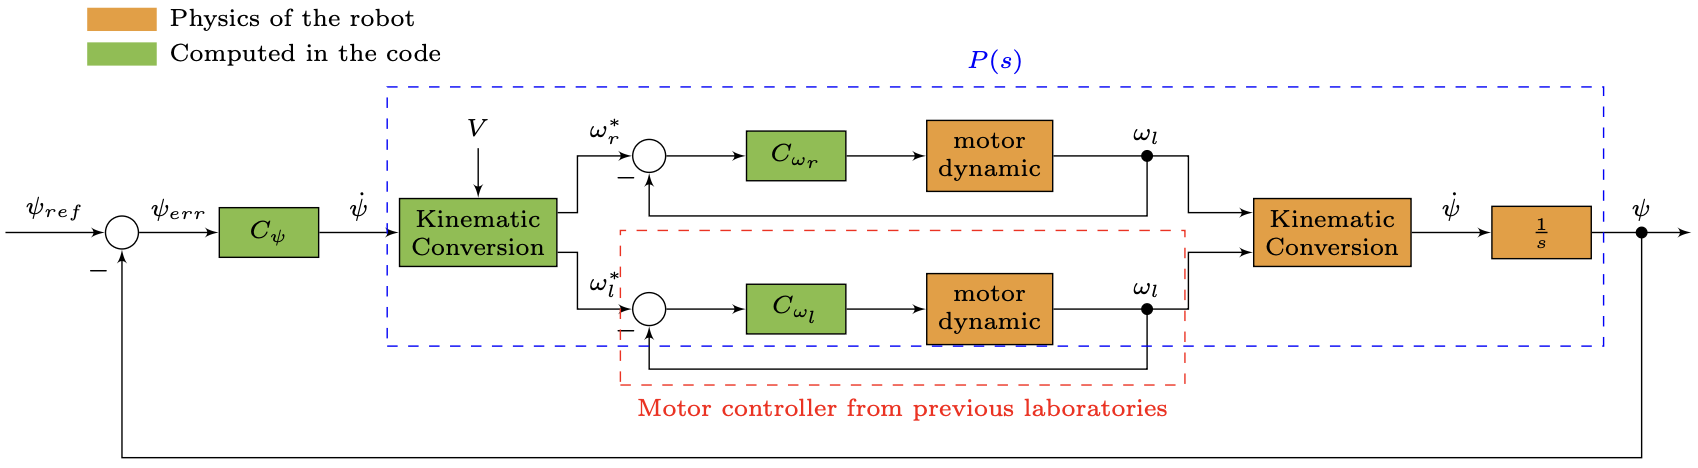
\includegraphics[width=0.7\textwidth]{lab4/figures/yaw_controller.png}
    \caption{Yaw controller}
    \label{fig:yaw_controller}
\end{figure}


\subsection{Code implementation}
\subsubsection{Implementation of the simple controller}
As initial approach we implemented a simple controller with the goal of keeping the robot on the line.
The controller was designed to to adjust the direction of the robot, by increasing the rotation speed of one wheel and decreasing the other, based on the readings of the line sensor array.

The global variables used in the code are shown in Code~\ref{lst:global}. 
These include the speeds of the motors (in RPM), reference values, control errors, and proportional-integral control terms for each motor. 
Gains Kp and Ki are used in the PI controller to regulate the motor speed based on the error. 
Variables are defined separately for motor 1 (controlled via timer 3) and motor 2 (controlled via timer 4).
\begin{lstlisting}[language=C, caption={Global variables}, label={lst:global}]
// motor 1
float TIM3_speed; // Speed of motor 1 in RPM
float reference_speed = 60; //RPM
float speed_error; 
static float u_int; // Integral term for speed control
float u_p; // Proportional term for speed control
float u_pi; // Proportional-Integral term for speed control
float Kp = 0.5;  // Proportional gain
float Ki = 6;    // Integral gain
uint32_t TIM3_CurrentCount;
int32_t TIM3_DiffCount;
static uint32_t TIM3_PreviousCount = 0;
float duty;

// motor 2
float TIM4_speed; // Speed of motor 2 in RPM
float reference_speed2 = 60; //RPM
float speed_error2;
static float u_int2; // Integral term for speed control
float u_p2; // Proportional term for speed control
float u_pi2; // Proportional-Integral term for speed control
float Kp2 = 0.5;  // Proportional gain
float Ki2 = 6;    // Integral gain
uint32_t TIM4_CurrentCount;
int32_t TIM4_DiffCount;
static uint32_t TIM4_PreviousCount = 0;
float duty2;
\end{lstlisting}

First of all, we checked the status of the line sensor, and we saved it in an array, where each element represents the status of a sensor (active [1] or not active [0]).
\begin{lstlisting}[language=C, caption={Status sensor line}, label={lst:sens_line}]
uint8_t sensor_line;
HAL_StatusTypeDef status_sens_line = HAL_I2C_Mem_Read(&hi2c1,
    SX1509_I2C_ADDR1 << 1, REG_DATA_B, 1, &sensor_line, 1, I2C_TIMEOUT);
for (int i = 0; i < 8; i++) {
    if ((sensor_line >> i) & 0x01) {
        active_pins[i] = 1;
    } else {
        active_pins[i] = 0;
    }
}
\end{lstlisting}
% TODO: check se codice c'è già nella parte del lab1

Next, inside the \texttt{HAL\_TIM\_PeriodElapsedCallback(TIM\_HandleTypeDef *htim)} function, we read the array \texttt{active\_pins} and we implemented the simple controller.
We decided to monitor only the pins on the far left (\texttt{active\_pins[0..2]}) and the far right (\texttt{active\_pins[5..7]}) to determine if the robot is drifting off the line.
Based on which pins are active, we adjust the reference speed of one motor to induce a turning behavior (see Code~\ref{lst:simple_alg}).
It is important to note that the \texttt{if} statements are not mutually exclusive, so if multiple conditions are satisfied, the last one overrides the previous ones.
This allows for a graded control based on how far the robot is from the center.
The logic focuses on turning by modifying only one of the two motors. For instance, if the robot needs to turn left, only the speed of motor 2 is increased, while motor 1 remains unchanged (default speed of 0 unless otherwise specified).
\begin{lstlisting}[language=C, caption={Simple algorithm}, label={lst:simple_alg}]
    //turn left
	if(active_pins[0])
		reference_speed2 = 10;
	else if(active_pins[0] && active_pins[1])
		reference_speed2 = 25;
	else if(active_pins[0] && active_pins[1] && active_pins[2])
		reference_speed2 = 37;

	//turn right
	if(active_pins[7])
		reference_speed = 10;
	else if(active_pins[7] && active_pins[6])
		reference_speed = 25;
	else if(active_pins[7] && active_pins[6] && active_pins[5])
		reference_speed = 37;
\end{lstlisting}

To compute the actual motor speed in RPM, we used the \texttt{\_\_HAL\_TIM\_GET\_COUNTER(\&htim3)} function to read the timer value. 
The RPM is calculated using the difference between the current and previous counter values, normalized with respect to the sampling time and the timer resolution.
We calculated the error between the reference speed and the current speed: \texttt{speed\_error = reference\_speed - TIM3\_speed;} for motor 1 and \texttt{speed\_error2 = reference\_speed2 - TIM4\_speed;} for motor 2. 
 This error is used in a PI (Proportional-Integral) controller to generate a control output, as shown in Code~\ref{lst:speed_control}.
The integral term accumulates the error over time, while the proportional term reacts to the current error. The final control output \texttt{u\_pi} is used to adjust the PWM duty cycle sent to the motor.
Note that the integral term \texttt{u\_int} is not bounded or clamped, which may lead to integrator windup if the error persists for a long time. This can be mitigated by adding saturation or anti-windup logic, though it's not implemented in this version.
\begin{lstlisting}[language=C, caption={Speed control}, label={lst:speed_control}]
    u_int = u_int + Ki * TS * speed_error;
    u_p = Kp * speed_error; 
    u_pi = u_int + u_p;     //Output of the PI controller
\end{lstlisting}

Finally, the PWM duty cycle is set using either the \textbf{Forward and Coast} method --- one motor terminal receives the PWM signal and the other is grounded. 
Alternatively, the \textbf{Forward and Brake} method can be used, where one terminal receives the PWM signal and the other is connected to the opposite voltage level, effectively shorting the motor terminals during the off-time. 
This provides active braking and allows for faster deceleration of the motor.
The duty cycle is calculated as a percentage of the maximum value, which is typically 100\% for full speed.
The final duty cycle is applied using the \texttt{\_\_HAL\_TIM\_SET\_COMPARE()} function, which sets the PWM output on the corresponding channel of the timer.
\subsubsection{Implementation of the yaw controller}
To the global variables defined in Listing~\ref{lst:global}, we added the following variables for the yaw controller:
\begin{lstlisting}[language=C, caption={Global variables for yaw control}, label={lst:global_yaw}]
float e_num,e_den,e_sl; // line tracking error
float psi_err; // yaw error
float V, w_1, w_2; // speed reference after the controller yaw
float kp_yaw = 7; // proportional gain for yaw control
float yaw_rate; 
float lambda[8]; // distance between the sensors and the center of the sensor array
\end{lstlisting}

As for the previous approach, inside the \texttt{HAL\_TIM\_PeriodElapsedCallback(TIM\_HandleTypeDef *htim)} function, we read the status of the line sensors and saved it in an array, see Listing~\ref{lst:sens_line}.
And we used it to compute the line tracking error $e_{SL}$, as shown in Listing~\ref{lst:line_tracking_error}, where we resorted to Equation (\ref{eq:lambda_n}), (\ref{eq:e_sl}) and (\ref{eq:psi_err}).
\begin{lstlisting}[language=C, caption={Line tracking error}, label={lst:line_tracking_error}]
e_num = e_den = 0;

for(int i=0;i<N;i++){
    lambda[i] = ((N-1)/2 - i)*P; // distance between sensor n and the center
    e_num += active_pins[i]*lambda[i]; // distance between sensor n and the center
    e_den += active_pins[i];
}
if(e_den == 0)
    e_sl = 0;
else
    e_sl = e_num / e_den;

psi_err = e_sl / H;
\end{lstlisting}

The yaw rate is calculated as a proportional term of the psi error as shown in Listing~\ref{lst:yaw_control}, which is then used to adjust the wheel speeds accordingly.
Indeed, we computed the desired wheel speeds $w_1$ and $w_2$ based on the reference speed and the yaw rate, using Equation~(\ref{eq:omega}), where the reference speed was set to 30 RPM.
Next, we used them to compute the speed error for each motor: \texttt{speed\_error = w\_1 - TIM3\_speed;} for motor 1 and \texttt{speed\_error2 = w\_2 - TIM4\_speed;} for motor 2.
\begin{lstlisting}[language=C, caption={Yaw control law}, label={lst:yaw_control}]
yaw_rate = kp_yaw * psi_err; 
V = (reference_speed*RPM2RADS)*r; //RADS
w_1 = ((V + yaw_rate*(D/2))/r)*RADS2RPM; // Right wheel speed
w_2 = ((V - yaw_rate*(D/2))/r)*RADS2RPM; // Left wheel speed
\end{lstlisting}

From now on, the code for the speed control of each motor is the same as in the previous approach, see Listing~\ref{lst:speed_control}.

\subsection{Results}
In this section we will present the results of the laboratory activity, focusing on the performance of the implemented line following algorithms.
We will analyze only the results obtained with the yaw controller, as it was the most advanced approach and yielded the best performance.

Figures~\ref{fig:yaw_controller_results_wheel_1} and \ref{fig:yaw_controller_results_wheel_2} show the performance of the yaw controller for Wheel 1 and Wheel 2, respectively, over a 6-second time window. 
For each wheel, five plots are reported:
\begin{itemize}
    \item the actual and reference wheel speeds,
    \item the speed tracking error,
    \item the control input (voltage) delivered to the motor,
    \item the resulting yaw rate (in rad/s),
    \item the yaw angle error (psi error, in rad).
\end{itemize}

\begin{figure}[H]
    \centering
    \begin{subfigure}{0.7\textwidth}
        \centering
        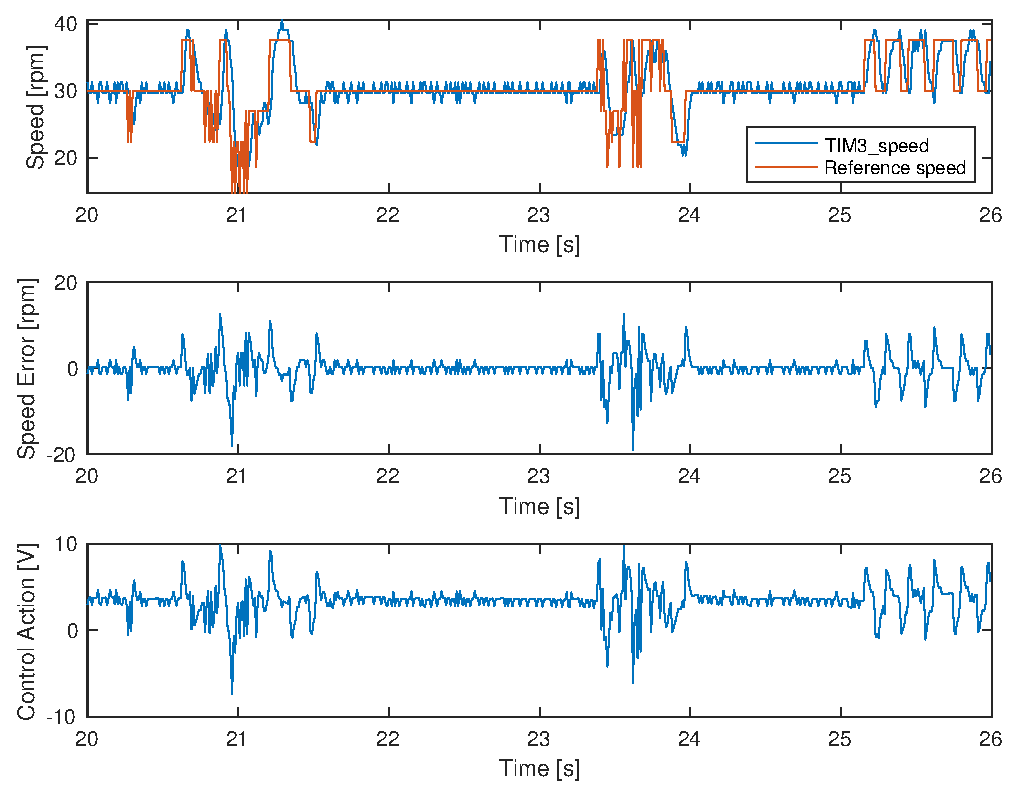
\includegraphics[width=\textwidth]{lab4/figures/wheel_1.eps}
    \end{subfigure}
    
    \vspace{0.5cm} % spazio verticale tra le due figure

    \begin{subfigure}{0.7\textwidth}
        \centering
        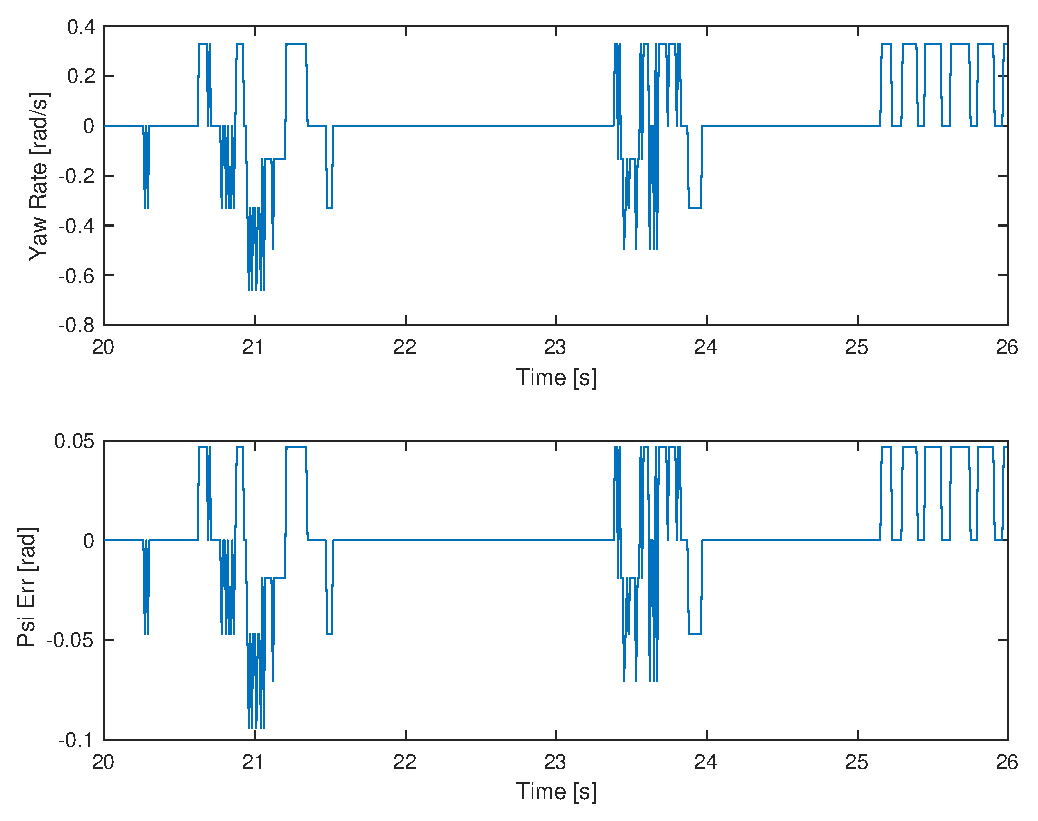
\includegraphics[width=\textwidth]{lab4/figures/yaw_1.eps}
    \end{subfigure}

    \caption{Yaw controller results for wheel 1}
    \label{fig:yaw_controller_results_wheel_1}
\end{figure}

From the first subplot, it is evident that the controller for Wheel 1 is able to track the reference speed with reasonable accuracy, especially during steady-state segments. 
Transient deviations occur when the reference signal changes abruptly, leading to observable overshoots and undershoots. 
These are reflected in the speed error plot, where oscillations are more pronounced in the initial and final parts of the time window.

The third subplot shows the control action in volts. 
The control signal remains mostly within the saturation limits of ±10V, indicating that the controller operates within feasible bounds. 
The presence of sharp control changes suggests that the system is responding to rapid reference changes or disturbances, consistent with what is expected in a dynamic line-following scenario.

The yaw rate plot demonstrates that the robot frequently adjusts its orientation to maintain the desired trajectory, with several peaks and zero-crossings indicating turns or corrections. 
Importantly, the psi error remains mostly bounded within ±0.1 rad, indicating effective heading control throughout the experiment.

\begin{figure}[H]
    \centering
    \begin{subfigure}{0.7\textwidth}
        \centering
        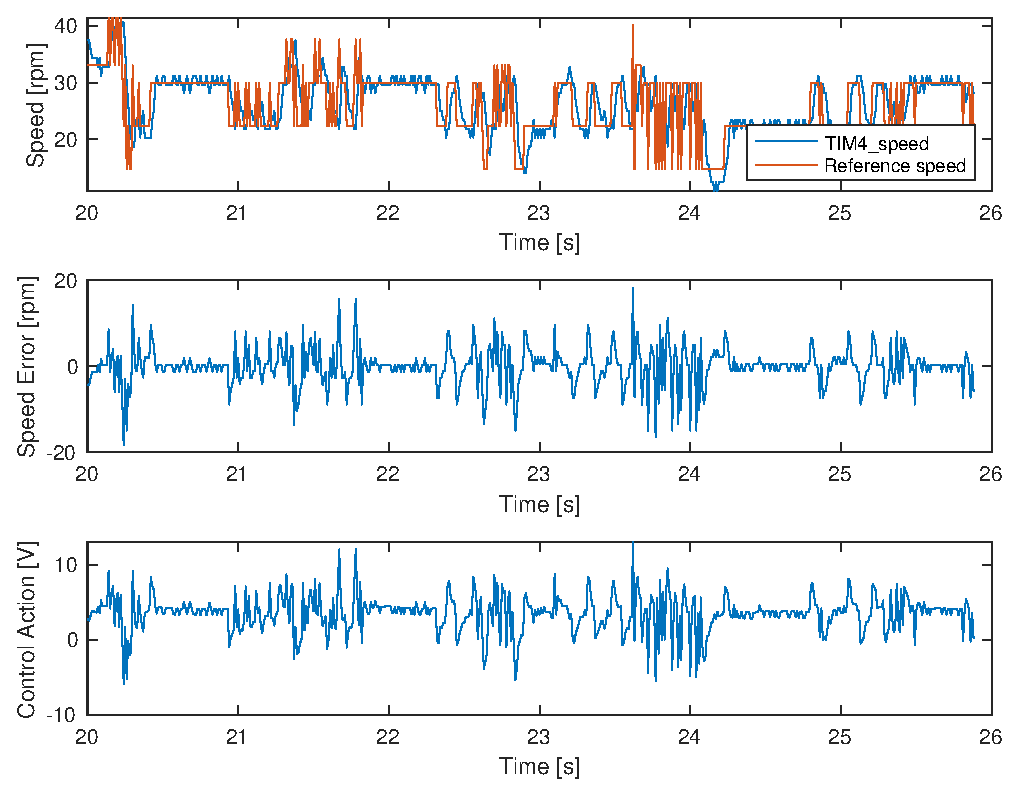
\includegraphics[width=\textwidth]{lab4/figures/wheel_2.eps}
    \end{subfigure}
    
    \vspace{0.5cm} % spazio verticale tra le due figure

    \begin{subfigure}{0.7\textwidth}
        \centering
        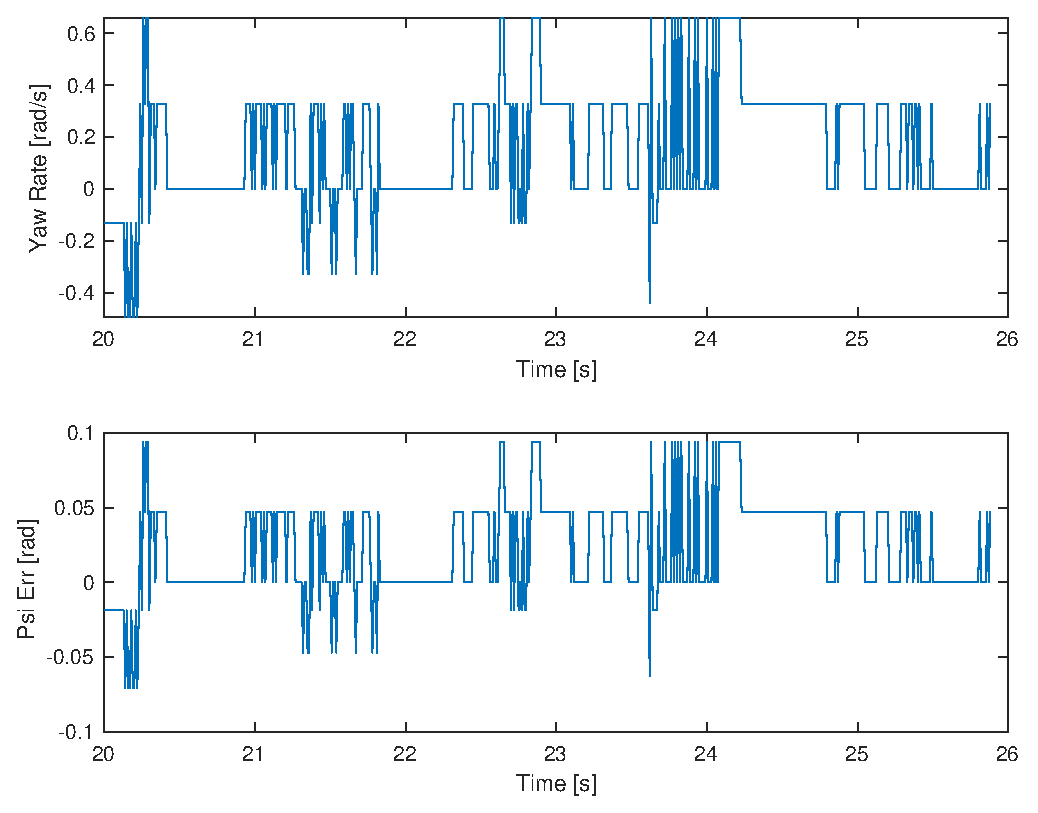
\includegraphics[width=\textwidth]{lab4/figures/yaw_2.eps}
    \end{subfigure}

    \caption{Yaw controller results for wheel 2}
    \label{fig:yaw_controller_results_wheel_2}
\end{figure}

The behavior of Wheel 2 follows a similar trend, although some differences can be observed. 
The reference tracking in the first subplot appears slightly more oscillatory, likely due to asymmetries in the mechanical response or load distribution. 
Moreover, the data collected for Wheel 1 and Wheel 2 corresponds to different simulations (due to the limited capacity of the datalogger), which may explain some of the discrepancies in the speed profiles.
The speed error is larger during some transitions, which translates to more aggressive control actions in the third subplot.

Despite this, the control voltage remains within saturation bounds and demonstrates good responsiveness. 
The yaw rate and psi error plots again confirm that the controller achieves continuous correction of orientation. 
Notably, psi error remains within the same tight bounds observed for Wheel 1, reinforcing the robustness of the overall yaw control strategy.

Overall, the yaw controller successfully maintains trajectory alignment by dynamically adjusting the individual wheel speeds. 
Both wheels contribute to heading correction, and the system demonstrates good performance in terms of responsiveness, error containment, and control effort. 
These results validate the effectiveness of the implemented controller in enabling stable and accurate line following under varying speed references and disturbances.

\subsection{Conclusion}
In this laboratory activity, we successfully implemented a line-following algorithm for the TurtleBot using a combination of low-level and high-level control strategies. 
The low-level controllers ensured precise wheel speed control, but the trajectory was not smooth, since the robot tended to oscillate around the line. 
To address this, we introduced a high-level yaw controller that adjusted the robot's heading based on the line tracking error. 
This approach significantly improved the robot's ability to follow the line smoothly and accurately. 
The results demonstrated that the yaw controller effectively minimized the yaw error, allowing the robot to maintain a stable trajectory.

We believe that further improvements can be made by tuning the controller parameters and increasing the velocities, which would allow the robot to follow the line more quickly while maintaining stability.